\documentclass[11pt]{article}
\usepackage[margin=0.85in]{geometry}
\usepackage{amsmath,amssymb,graphicx,hyperref}
\setlength{\parindent}{0pt}\setlength{\parskip}{7pt}
\setlength{\emergencystretch}{3em}
\begin{document}
{\Large Testing a sparse differential norm filter}\\
November 13, 2026. Unsigned producer evidence [pcc:unverified].

\textbf{Algorithmic proposal.} Replace matching $N=cG$, where $N=A^2-fB^2$,
by the sparse derivative/convolution equation
\[
 W_G(N):=G N'-G'N=0.
\]
The test asks whether this adds useful constraints and whether finite
characteristic permits false positives. This is an exact algebraic test,
not a timing or empirical scaling campaign.

\textbf{Exact result.} Over any field, suppose $G$ is monic,
$\gcd(G,G')=1$ and $\deg N\leq\deg G$. Then
\[
 W_G(N)=0\quad\Longleftrightarrow\quad N=cG\text{ for some scalar }c.
\]
If $N\ne0$, then $c\ne0$. The theorem applies to the actual polynomial norm
lift with the stated degree cap. Products of distinct node factors $X-x_i$
satisfy monicity and coprimality; the usual norm pole-degree inequalities
supply the cap. No assumption $p>\deg G$ is needed.

\textbf{Proof mechanism.} The filter equation implies $G\mid G'N$.
Coprimality gives $G\mid N$; the degree cap and monicity force a scalar
quotient. Conversely, differentiating $cG$ gives the zero filter.

\begin{center}
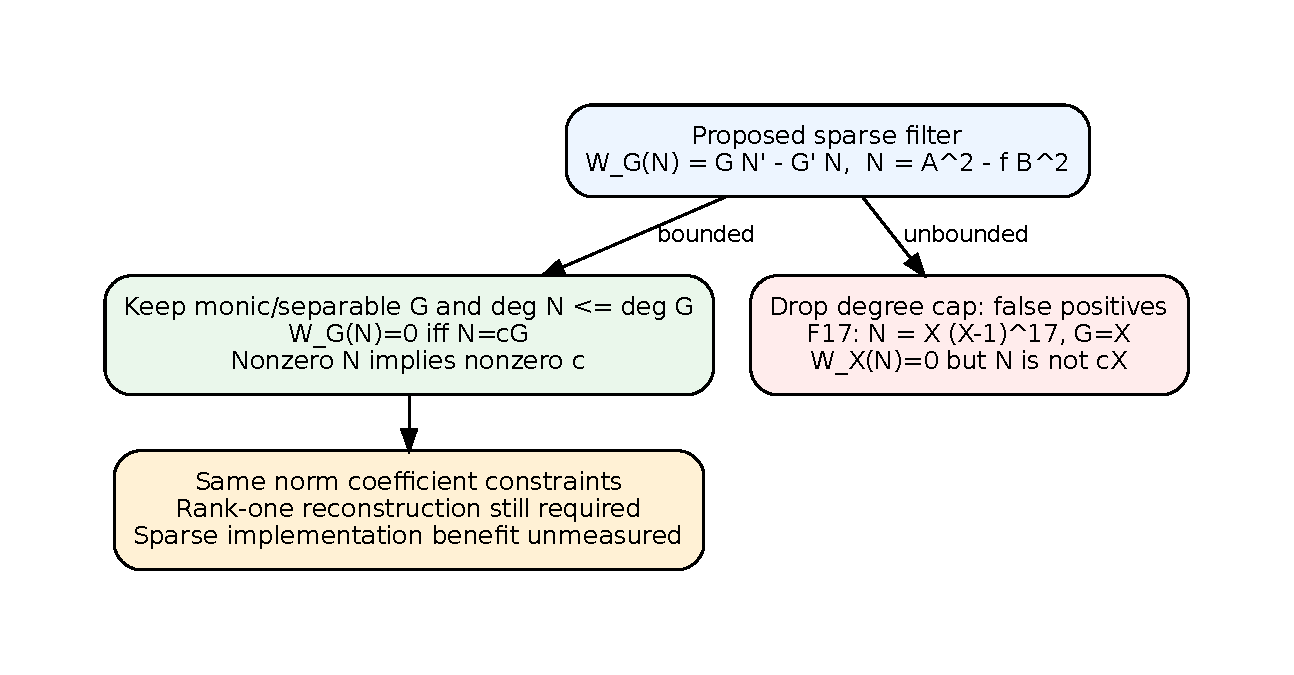
\includegraphics[width=0.96\linewidth,height=0.34\textheight,keepaspectratio]{filter.pdf}
\end{center}

\newpage
{\Large Finite-characteristic check and research disposition}

\textbf{False positives without the cap.} Over $\mathbb F_{17}$,
$W_G(GH^{17})=0$ for every $G,H$, since $(H^{17})'=0$.
The explicit nonzero polynomial $N=X(X-1)^{17}$ passes $W_X$ but is not
$cX$: evaluation at1 would give $c=0$, while evaluation at2 contradicts
that value. Lean checks both the passing filter and non-proportionality.
This fixture tests the polynomial filter, not an ECDLP target solve.

\textbf{What was learned.} Within the genuine degree window this is exactly
the original scalar norm condition. It is not stronger pruning and does not
remove rank one. Outside the window it can accept incorrect candidates.
Kernel equivalence alone does not rule out a sparse implementation benefit;
none was measured. In particular,
\[
 (A^2-fB^2)'=2AA'-f'B^2-2fBB'
\]
still depends quadratically on the unknown coefficients. A linear routine
returning $N=cG$ has not constructed $A,B$.

\textbf{Formal map.} In module \path{NormWronskian}, the kernel theorem is
\path{filterZeroIff} and the actual-lift corollary is \path{liftedFilterIff}.
The README maps all ten statements to their exact hypotheses and canonical
unsigned bindings in the evidence directory.

\textbf{Evidence.} Source commit \path{923a40182}; Lean4.35.0 with unchanged
pinned dependencies. Default build004 passed3145 jobs. Actual tracked-source
gate passed39 declarations with zero additional trusted axioms. Failed
builds001--003 are preserved; they involved the finite-field instance and
natural-number casts. All final printed foundations are standard.
Import-inclusive replay status is retained in the evidence directory.

Native identity record \path{IDC1hd9711b7c88619f6b} binds the expanded residual
and source hash. The existing issuer/checker accepted32 statement-derived
and32 extra stream points. It does not execute Lean or establish an algorithmic
bound; the universal kernel theorem and F17 implications are checked separately.

\textbf{Next research target.} Nonlocal rank-one reconstruction exploiting the
coupled Hankel coefficient structure. No such search routine or time bound is
provided here. This test does not exclude the whole norm approach.

\textbf{Sources and resources.} Pinned Mathlib derivative, separability,
coprimality and monic-degree lemmas; recorded Galbraith norm references;
the barrier map's p-adic scope. KB unavailable, so no novelty claim.
The monthly isolab budget is recorded exhausted; no paid experiment,
benchmark row, timing comparison or historical graph change was made.
\end{document}
